\subsubsection*{Survey Methodology} \label{sec:methodology}
    While theoretically a two-way trust model could be considered (i.e. in which the AIA also has trust in the user), attention is restricted here to a one-way trust relationship that considers only how user trust (and TRBs) evolves in response to assurances from the AIA. 

    It should be noted that it is practically impossible to perform a fully comprehensive survey of all AIA assurances, due to the broad spectrum of possible assurances, and AIAs in general. As an example, one could rightly argue that control engineers treat metrics like gain and phase margins as assurances for automatic feedback control systems, in much the same way that machine learning practitioners treat training and test accuracy as assurances for learning algorithms---and hence concepts related to robustness, stability, etc. for feedback control systems ought also be included in this survey. Similar arguments for assurances developed for fields like econometrics, software testing, aeronautical engineering and many others. While assurances can, in theory, be applied in both the most simple `automatic' systems (like a thermostat), this survey will focus on assurances in more advanced AIAs that make decisions under uncertainty. However, the admittedly narrow scope of this survey does not impede the development of fundamental insights and principles in designing assurances.

    Initially, in order to find applicable research, papers that formally addressed trust, and tried to create models of it, were investigated. This was done with the aim of trying to understand how trust might be influenced. Secondly, literature regarding trust between humans and some form of machine entity was reviewed; this lead to research in fields like e-commerce, automation, and human-robot interaction. Third, research on `interpretable', `comprehensible', `transparent', `explainable', and other similar types of learning and modeling methods were examined. Finally, with that literature as a background, research disciplines investigating computational methods that can be useful as assurances, but in which trust itself is not the main focus, were considered. This information was then used to construct an informed definition and classification of assurances based on methods that are currently in use, or being investigated.
    
    We now proceed to discuss each of the categories from Figure~\ref{fig:assurance_continuum}, starting from the most integral to the AIAs core functionality and proceeding to the least integral.


\section{A Survey of Assurances} \label{sec:survey}
Now that AIA, trust, TRBs, and assurances have been defined we are ready to begin the survey of assurances. There are many different ways in which this survey could be organized, we choose to present it based on the different goals of the main groups of researchers who have been working in the area.

Early in reading the related literature it became clear that there were two main groups: 1) those researchers who have formally addressed the topic of trust between humans and AIAs of some form, and 2) a much larger body of those who have informally considered trust in their work. Here we consider formal treatment of trust to include those who acknowledge a human trust model and who gather data from human users in order to measure the effect of assurances on trust. Informal treatment of trust includes those who reference the concept of trust, but who do not gather user data to verify the effects of proposed assurances. 

Another way that the landscape of researchers might be divided is by the kinds of assurances they investigate. The first group consider what we call `implicit' assurances. Implicit assurances embody any assurances that are not deliberately designed into the AIA. The second group consider `explicit' assurances; which are assurances that were explicitly created by a designer with the intent of affecting a user's trust. Implicit assurances can be thought of side-effects of the design process; for example HAL 9000 could have been designed with a circular `red-eye' looking sensor because it was cost-effective, however it is possible that users who interact with HAL might find the `red-eye' sensor to be a bit creepy, and thus lose trust in HAL. Conversely, the same `red-eye' may have been explicitly designed and selected based on several studies that indicated that users find it easier to trust advanced AIAs with `red-eye' sensors instead of similarly shaped green sensors.

Much of the research that formally considers trust has focused on implicit assurances. This is likely due to the focus on investigating what properties of an autonomous systems can affect a user's trust. It is possible to argue that someone who finds that reliability affects a user's trust is investigating an explicit assurance, but for the purposes of this paper we try to stay true to the intent of the researcher when performing the work. More recently, as seen by a large spike in interest in `interpretable', and `explainable' AIAs in government, academic, and public circles, we have seen an emergence a group who acknowledge that the concept of trust in human-AIA relationships, and who want to design systems accordingly.

In view of these four main groups of researchers, we organize the survey by creating four quadrants shown in Figure~\ref{fig:trust_assurance_intention}. In the remainder of this section we survey each of these quadrants separately in order to gain some understanding of the lessons that each has to offer when we consider the design of assurances.

\begin{figure}[htbp]
    \centering
    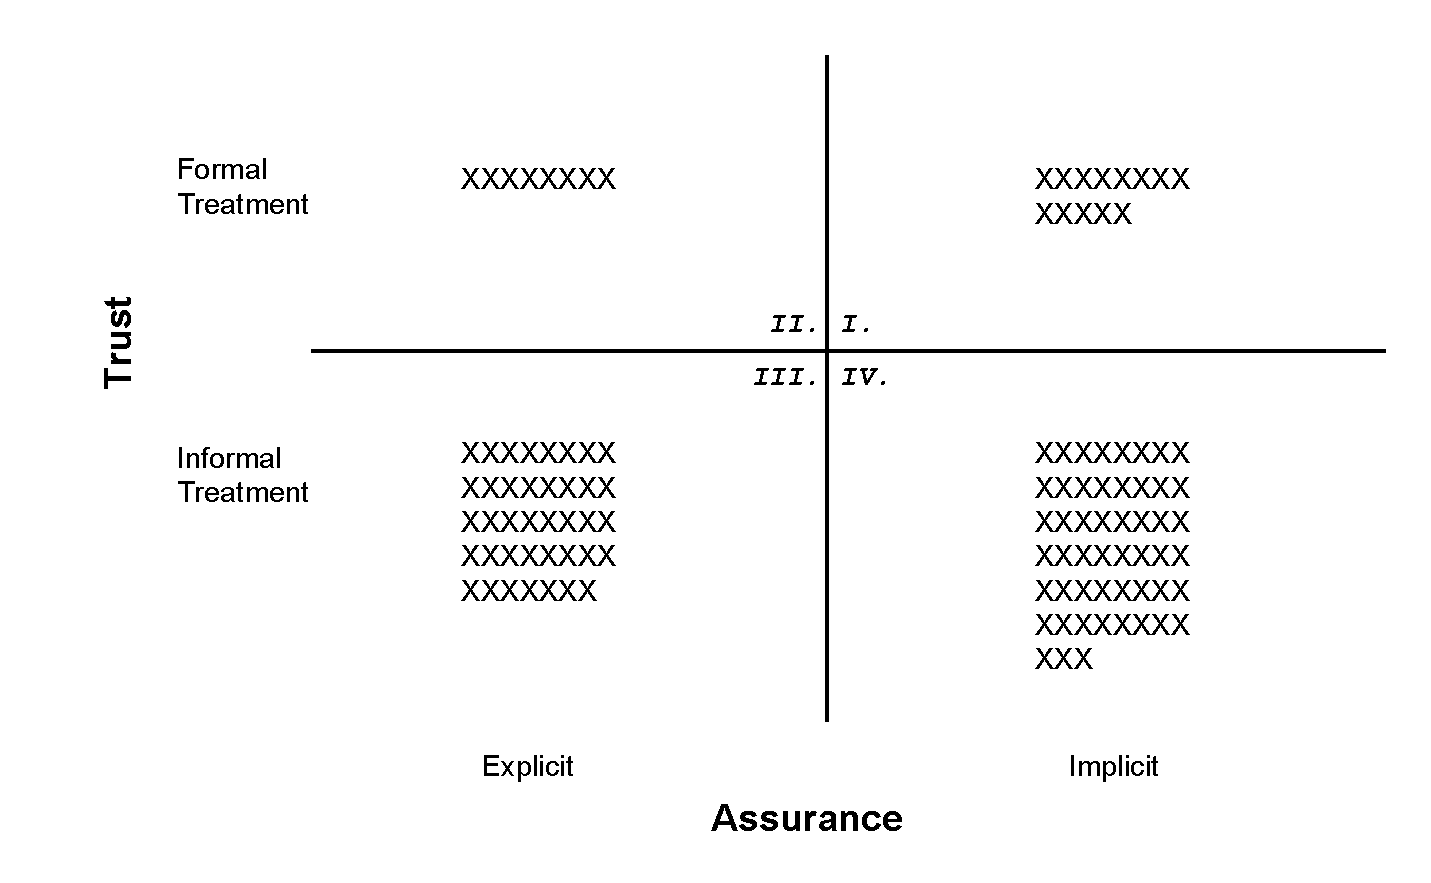
\includegraphics[width=0.8\textwidth]{Figures/Trust_vs_Assurance_Intention.pdf}
    \caption{Figure depicting how many papers consider trust both formally and informally, as well as those who investigate explicit and implicit assurances}
    \label{fig:trust_assurance_intention}
\end{figure}

\begin{itemize}
    \item \hyperref[sec:q1]{Quadrant I.} (implicit assurances, formal trust treatment) -- Gather user data, consider a trust model, consider assurances that are implicit (i.e. those who care about human-AIA trust, but aren't designing assurance algorithms)
    \item \hyperref[sec:q2]{Quadrant II.} (explicit assurances, formal trust treatment) -- Gather user data, consider a trust model, consider assurances that are explicit (i.e. those who formally acknowledge human-AIA trust, and design assurances to affect it)
    \item \hyperref[sec:q3]{Quadrant III.} (explicit assurances, informal trust treatment) -- Do not gather data from users, reference trust (or its components interpretability, etc..), consider assurances that are explicit (i.e. those who know that the concept of `trust' is important, but that only use an informal notion of it when designing assurances)
    \item \hyperref[sec:q4]{Quadrant IV.} (implicit assurances, informal trust treatment) -- Not interested in affects on user trust, but reference (possibly only allude to) concepts that are related to trust as defined in this paper. Investigate approaches for creating AIAs with improved properties or characteristics. (i.e. those whose work is relevant for designing assurances, but don't know it)
\end{itemize}

\subsection{Quadrant I. (Implicit Assurances, Formal Trust Treatment)}\label{sec:q1}
\citet{Muir1996-gt} performed an experiment where participants were trained to operate a simulated pasteurizer plant. During operation they were able to intervene in the fully-autonomous system if they felt is was necessary to obtain better performance. Trust was quantified by self-reported questionnaire responses, as well as by the level of reliance on the automation during the simulation. She noted that operators could learn to trust an unreliable system if it was consistent. The participants were only able to observe the reliability of the pump (i.e. the performance of the pumps over time, from which the user created a mental model of reliability).

In experiments involving thirty students and thirty-four professional pilots, \citet{Riley1996-qm} investigated how reliability and workload affected the participant's likelihood of trusting in automation. Two simulated environments were created to this end. First was for participants to use/not use an automated aid (with variable reliability) to classify characters while also performing a distraction task. Interestingly, they found that pilots (those with extensive experience working with automated systems) had a bias to use more automation, but reacted similarly to students in the face of dynamic reliability changes. In this setting, the bias to use more automation would be known as `framing effects' (where a human's trust is biased by the trust they have in previously encountered systems) in cognitive science. Findings also showed that the use of automation is highly based on individual traits.

Also considering the performance of pilots, \citet{Wickens1999-la} investigated the effect of semi-reliable data while piloting a plane. They also investigated semi-reliable performance of a system that highlighted important data for the pilot to see. The pilots were aware that the measurements/highlighting system might be inaccurate before the experiment. The reliability of the systems did have an effect on the outcome of the experiment, but interestingly did not make a measurable effect on the pilot's self-reported trust. This underscores the point that TRBs ought to be the focus of assurances as opposed to trust itself, since trust is a subjective measure that may or may not actually change a person's TRBs.

McKnight and collaborators have spent significant time investigating trust between humans and technology. His initial research was focused on e-commerce settings but later moved to trust between humans and technology. In \cite{Mcknight2011-gv} they gather self-reported trust through a questionnaire. Their experiment was interested in identifying the dimensions of trust effected by learning to use Excel for use in a business class. The results were based solely on the intrinsic properties of excel and how each individual perceived them.

In \cite{Lankton2008-ct} and later in \cite{Tripp2011-rx} they investigate the difference in trust between humans and trust between a human and technology. They found that as the technology becomes more `human-like' the self-reported trust has more similarities to trust between humans. This study was performed using Microsoft Access, a recommendation assistant, and Facebook. Respondents were asked to rate how each software `kept its commitments' and how `human-like' it was. Again, these impressions were based solely on the intrinsic properties of each of the three AIAs used in the experiment.

\citet{Freedy2007-sg} studied how `mixed-initiative teams' (MITs, their term for human-robot teams) might have their performance measured. The premise of the work is that MITs can only be successful if ``humans know how to appropriately trust and hence appropriately rely on the automation''. They explore this idea by using a tactical game where human participants supervised an unmanned ground vehicle (UGV) as part of a reconnaissance platoon. UGVs had three levels of capability (low, medium, high), and had autonomous targeting and firing capability which the operator needed to monitor in case the UGV could not perform as desired. Operators were trained to recognize signs of failure, and to only intervene if they thought the mission completion time would suffer. Trust was formally acknowledged in this survey and was quantified by using Relative Expected Loss (REL), which is the mean expected loss of robot control over $n$ trial runs. Operators were found to be more likely to use a `medium' ability UGV if they had first encountered a `high' ability UGV, as opposed to encountering a `low' ability UGV first, which is another manifestation of framing effects like \cite{Riley1996-qm}. Similar to \cite{Muir1996-gt} the operators learned to trust a UGV with low competence as long as it behaved consistently. \edit{make sure REL is explained well}

In a similar vein \citet{Desai2012-rc} investigated the effects of robot reliability on the trust of human operators. In this case a human participant needed to work with an autonomous robot to search for victims in a building, while avoiding obstacles. The operator had the ability to switch the robot from manual (teleoperated) mode, to semi-autonomous, or autonomous mode depending on how they thought they could trust the system to perform. During this experiment the reliability of the robot was changed in order to observe the effects on the operator's reliance to the robot. Trust was measured by the amount of time the robot spent in different levels of autonomy (i.e. manual vs. autonomous), and it was found that trust changed based on the levels of reliability of the robot.

\citet{Salem2015-md} investigated the effects of error, task type, and personality on cooperation and trust between a human and robot. In this case the robot was a domestic robot that performed tasks around the house. A human guest was welcomed to the home and observed the robot operating on different tasks. After this observation (in which the robot implicitly showed competence by its mannerisms and successes/failures) the human participant was asked to cooperate with the robot on certain tasks. Interestingly, it was found that self-reported trust was affected by faulty operation of the robot, but that it didn't seem to have an effect on whether the human would cooperate on other tasks. This seems to suggest that the effect of institutional trust (i.e. this robot may not be competent, but whoever designed it must have known what they were doing) allowed users to continue to cooperate with a faulty system, even if they have low levels of trust in it.

\citet{Wu2016-ei} use game theory to investigate whether a person's decisions are affected by whether they believe they are playing a game against a human or an AI. This idea was studied in the context of a coin entrustment game, in which trust is measured by the number of coins a participant is willing to lose by putting them at risk of the other player. On the surface, their work is meant to be a study of the implicit differences in trustworthiness between humans and robots; however in their experiment the `human' was actually an AI with some programmed idiosyncrasies to lead the human player to believe the AI was a human. This was done by adding a random wait time, as opposed to an instantaneous move that the AI would make. There were also prompts at the beginning of the `human' version of the experiment that suggested that the participant was waiting for another human player to join the game. The experiment found that humans trust an AI more than they trust a `human'. The authors suggest that this may be due to the perception that an AI does not have feelings and is operating in a more predictable way. Given that the `human' was an algorithm as well, this experiment shows that consistency (i.e. no variable wait times) was a factor that affected the trust of the participant.

\citet{Bainbridge2011-pl} investigated the difference in trust between a human and a robot, in cases where the robot was physically present and where the robot was only displayed on a screen (i.e. not physically present). In this experiment, the only method of communication from the robot was through physical gestures. Trust was measured by the willingness of the human participants to cooperate with the robot. Among other interesting findings regarding how the participants interacted with the robot, it was found that participants were more likely to cooperate with the robot when it was physically present. \citeauthor{Bainbridge2011-pl} suggest that this is due to increased trust, in this case cooperation is a TRB.

With the aim of understanding how individuals currently trust autonomous vehicles, \citet{Munjal_Desai2009-en} performed a survey of around 175 participants. The participants were asked to rate their level of comfort with six different situations. These situations ranged from parking your own car, having an autonomous vehicle with manual override park the car, and having a fully autonomous vehicle that could not be overridden park the car. There were also questions related to user comfort with autonomy in situations where they still retained control, like how comfortable users would be with having autonomous vehicles park near their car. The survey found that the participants were most comfortable with parking their own car, and least comfortable with having a fully autonomous vehicle (with no manual override) park their car. These findings are supposedly related to institutional trust, as those surveyed did not necessarily have any experience with autonomous vehicles.

\subsubsection{Summary}
There have been several experiments that have formally shown that implicit assurances have an effect on a user's trust towards an AIA. Generally these findings have been accompanied by the advice that designers should consider that trust is an important element and can affect user's behavior towards an AIA. 

Generally intrinsic assurances can affect any of the three key trust dimensions (from Figure~\ref{fig:Assurance_classes}). To speak more specifically, reliability (or rather the perception of reliability built over contiguous observations) was frequently used in this section. A reliable AIA seems more competent, and predictable to a human user. This is to say that there are not inherent limitations on intrinsic assurances that limit the dimensions of trust that they can affect.

Generally this body of work investigates what kinds of properties of AIAs affect the trust of human users. We see some evidence for the idea that a user will gather assurances, whether these are implicit or explicit, in order to execute TRBs. That is to say that in the absence of explicitly provided assurances a user will still use other perceived properties and behaviors and gather assurances in order to inform their trust-related behaviors.

Even if an AIA has the capability to calculate an assurance, it must still have a way by which to express that assurance to a human user. The human user then perceives the assurance, perhaps through interaction with the system, or only from observation of the system. These kinds of perceptions can be based on displayed information, or on how the AIA `behaves' (as in \cite{Salem2015-md}). Once the user perceives some kind of assurances (perhaps not purposefully communicated), those assurances are integrated into the trust of the user towards the AIA. In most cases the surveyed research focuses on assurances given through sight, but sound and touch cannot be totally discounted because they may likely have played a part in some of the interfaces between the humans and AIAs. 

We also see evidence that human cognitive limitations need to be taken into account when designing assurances. This was directly observed in \cite{Freedy2007-sg,Riley1996-qm} where framing effects biased operators decisions. This also suggests that other cognitive limitations such as `recency effects' (biased based on recent experience), and others likely apply. Another limitation is the time required for humans to build statistical models, such as reliability, when only instance by instance data is available.

From this research we are able to get a feeling for what indicates changes in trust, and how it should be measured. Specifically: through measuring different actions, called TRBs in this document, and through self-reported changes in perceived trustworthiness. Implicit assurances are not targeted at specific trust dimensions. It seems, that except in a very controlled environment, that they originate from several different sources of AIA capabilities at once, as they are only based on a user's perception and would be unconsciously combined into an overall `sense' of trustworthiness.

\subsection{Quadrant II.}
Muir investigated explicit assurances that automation could give to human operators in order to affect trust. She began by investigating formal models of trust between humans and then extending those concepts to trust between humans and automation. In \cite{Muir1987-mk} and \cite{Muir1994-ow} she investigated how decision-aids could be designed in order to affect trust. Within the framework of a trust model she suggested that a user must be able to ``perceive a decision aid's trustworthiness'', which could be accomplished by providing data regarding the system's competence on a certain task. She also suggests that summary information regarding the system's reliability over time would help. Finally she suggests improving the ``observability'' of the machine behaviors so that the user can understand it more fully.

She goes on to suggest that the user must have an accurate criteria for evaluating the system's trustworthiness. This would involve understanding the domain of competence, the history of competence, and criteria for acceptable performance of the system. She also suggests that a user must be able to allocate tasks to the system in order to feel equal in the trust relationship. The idea is that a relationship in which only one entity makes decisions is not amenable to calibrated trust. Finally she suggests that it is important to identify and `calibrate' areas where a user may trust the system inappropraitely. One key shortcoming of her work is that she suggests types of explicit assurances, but does not suggest concrete approaches to implement them, or test them by experimentation.

\citet{Dragan2013-wd} investigated how a robot could move in a `legible' way, or in other words, make movements that in themselves convey the intended destination. They investigate this within the context of how quickly a human participant is able to predict the goal of a moving point, before the point actually reaches that goal. They found that legible motion does in fact improve the user's ability to understand and predict where the robot is trying to move. It is difficult to classify this work because it does not directly address or consider human trust, but it is clearly an explicit motion-predictability assurance. Furthermore, they run human experiments in order to validate that the calculated motions are in fact more interpretable to users. \nisarcomm{How generalizable or extensible are their ideas to other domains of AIA capabilities, i.e. perception, reasoning, etc. -- are they only limited to talking about physical motion? Is this a limitation of their work?}

\citet{Kaniarasu2013-ho} examine whether or not misuse and disuse (over and under trust, in their terminology) can be detected and the calibrated (aligned) to be within its competence. They use data from an experiment of a robot with a confidence indicator in a user interface. A user was asked to provide trust feedback every twenty seconds while operating a robot along a specified path without hitting obstacles and responding to secondary tasks. The user was able to switch between partially autonomous and fully autonomous modes. The experiment indicated that indicators of confidence did in fact reduce misuse and disuse. \nisarcomm{HOW was the confidence computed? Is this a generalizable method? }

Although they don't perform an experiment \citet{Chen2014-dk} lay out a framework that is based in formal trust models. The aim is to make the situation and agent more transparent to a collaborative human user. They propose explicit feedback that can support the three levels of an operator's situational awareness (SA). They call their model the SA-based Agent Transparency (SAT) model. The first level -- Basic Information -- includes understanding the purpose, process, and performance of the system. The second level -- Rationale -- includes being able to understand the reasoning process of the system. The third level -- Outcomes -- involves being aware of future projections and potential limitations of the system. They suggest that two main components are display of information, and the display of uncertainty, but note that there are many considerations to take into account when trying to communicate information to human users. For example, numerical probabilities can be confusing and may need to be replaced by confidence limits or ranges. \nisarcomm{again, talk about impact and limitations/open questions}

\citet{Chadalavada2015-wx} investigated way to make interaction between humans and robots more natural in a setting where they may occupy the same work space. Their approach was to have the robot project its intended movements onto the ground in order to indicate where it would be moving. They performed experiments in which participants were asked to answer questionairres regarding how predictable, reliable, and transparent the robot was when it was projecting its intentions, and when it wasn't. There was a significant improvement in all measures when the robot was projecting its intended movements. \nisarcomm{again, talk about impact and limitations/open questions}

\citet{Wang2016-id} investigate how explanations of robot reasoning can effect human-robot trust as measured by subjective questionnaires. In their experiment a human and robot need to investigate a town; the robot has sensors that detect danger, and will recommend that the human wear protective gear if it senses danger. However, the human may choose to not accept the recommendation based on their trust in the robot, and the need to avoid the delay associated with using the protective gear. The robot is able to pose natural-language explanations for its recommendations, as well as report its ability. They used explanations generated by components of the robot's planning model (the robot uses a partially observable Markov decision process (POMDP) planner). This allowed it to make statements like: ``I think the doctor's office is safe'', or ``My sensors have detected traces of dangerous chemicals'', or ``My image processing will fail to detect armed gunmen 30\% of the time''. They found that when the robot's ability was low, the explanations helped build trust. Whereas, when the capability was high, the explanations didn't have a significant effect. \nisarcomm{again, talk about impact and limitations/open questions of this approach}


Also regarding a robot with POMDP planning and actions, \citet{Aitken2016-fb} and \citet{Aitken2016-cv} consider a formal model of trust, and propose a metric called `self-confidence' that is a composite assurance for a robot that uses a POMDP for action. There are five component assurances that make up the composite: 1) Model Validity, 2) Expected Outcome Assessment, 3) Solver Quality, 4) Interpretation of User Commands, and 5) Past Performance. 

Self-confidence is reported as a single value between $-1$ (complete lack of confidence), and $1$ (complete confidence). A self-confidence value of $0$ reflects total uncertainty. Each of the component assurances would be useful on its own, but the composite is meant to distill the information from the five different areas so that a (possibly novice) user can quickly, and easily evaluate the confidence of the robot to perform in a given situation. Currently only one of the five algorithms (Expected Outcome Assessment) has been developed, but there is continuing work on the other metrics. As of the writing of this document no human experiments have been performed to validate the effect of the self-confidence metric.

Finally, \citet{Wu2016-ei} use game theory to investigate whether a person's decisions are affected by whether they believe they are playing a game against a human or an AI. This idea was studied in the context of a coin entrustment game, they measure trust as the number of coins a participant is willing to put at risk. On the surface the paper is meant to be a study of the implicit differences between humans and robots, however in their experiment the `human' was actually an AI with some programmed idiosyncrasies to lead the human player to believe the AI was a human. This was done by adding a random wait time, as opposed to an instantaneous move that the AI would make. There were also prompts at the beginning of the `human' version of the experiment that suggested that the participant was waiting for another human player to join the game. The experiment found that humans trust an AI more than they trust a `human'. The authors suggest that this may be due to the perception that an AI does not have feelings and is operating in a more predictable way. Given that the `human' was an algorithm as well, this experiment shows that consistency (i.e. no variable wait times) was a factor that affected the trust of the participant. Since this behavior was explicitly added to the logic it is a planning-predictability assurance. \nisarcomm{again, talk about impact and limitations/open questions of this approach -- e.g. could/have such approaches be extended to things like designing perception or learning assurances, or is this an open question? }

\subsection{Quadrant III. (Explicit Assurances, Informal Trust Treatment)}\label{sec:q3}
\subsubsection{Performance Prediction} \label{sec:performance_prediction}
    \citet{Zhang2014-he} are concerned with the performance of vision systems; particularly with the common occurrence of vision systems to fail `silently', that is with no warning. They suggest that the two possible solutions are to: 1) analyze the output of the vision system to assess its confidence, and 2) analyze the input itself in order to assess the classifier's confidence. They pursue the second, with the goal of minimizing failures as well as trying to verify the safety of a classifier. They argue that the second method is more desirable because it can be applied to any classifier. In essence they learn a model of the training error associated with different images and then use this to predict the error on test images. They demonstrate their methods on several different classification tasks and show that it predicts failure ``surprisingly reliably''. Although, they make an assumption that similar inputs (by some measure) will give similar outputs, this seems like it may be difficult to quantify in some domains.

    \citet{Gurau2016-hs} (following from ideas in \citet{Churchill2015-ei}) consider the task of predicting the performance of a robot's navigation when using cameras for localization. Their aim was to have the robot operate autonomously only when it was confident that it could do so, otherwise it would request human assistance. To achieve this they make use of GPS localized observations and `Experience Based Navigation' (EBN) to identify which past experience matches the current state of the robot. Using this approach they are able to reduce the number of mistakes that the robot makes when navigating in a real scenario. This approach seems to be fairly sound in their suggested application, and they claim that it is agnostic of classifier, which should be beneficial for use in other AIAs.

    \citet{Kaipa2015-hy} also consider the confidence of a visual classifier, but with the application being a robot that is picking an object out of a bin. To do this they utilize the `Iterative Closest Point' (ICP) method to match which points in a point cloud are likely associated with the object of interest in the bin. With that information the robot can then asses how confidently it can perform the task and if its confidence is below some threshold it will request assistance from a human. This method is quite similar to `Chi-square innovation hypothesis testing' used for adaptive Kalman filtering \cite{Bar-Shalom2001-tg}, and shares a key drawback, which is that it requires a precise model, and doesn't necessarily indicate \emph{why} the test is failing. Regardless, if applicable they are quite useful for verifying that the AIA is `OK'.

    \citet{Kuter2015-qh} recognize that plans can be fragile, and suggest that the planner calculate its stability. That is to say, how sensitive is the plan to uncertainties? They suggest `counter planning' and `plan repair' so that the autonomous system can identify likely contingencies that might interfere with an existing plan and then adapt the plan to account for those contingencies. If the system \emph{is} able to adapt to contingencies then it will have a higher `self-confidence'. This allows humans to be able to understand the system better, and trust it more appropriately.

    \citet{Hutchins2015-if} consider the fact that autonomous systems have components, and that those components have `competency boundaries'. That is to say that different sensors, planners, and actuators have different capabilities in different conditions. For example a GPS has high competency in an open-air situation, but very low competency inside of a tunnel or building. They suggest that these competency boundaries be quantified, and then displayed to a user, so the user better understands the system's capabilities and can trust it more. The main limitation here is that they propose an expert-based Likert scale for quantifying competency boundaries, which, which  lacks formal foundations, and extensions to other domains. Both this work and that of \citeauthor{Kuter2015-qh} are related to the work of \citeauthor{Aitken2016-fb}, but the later two do not explicitly relate their approaches to trust and TRBs. Although, \citeauthor{Hutchins2015-if} is the only paper of the three to consider the exact method by which the assurance should be communicated.

\subsubsection{Interpretable Models} \label{sec:model_interp}
    A well-known concept in machine learning and pattern recognition is the trade-off between accuracy and interpretability. \citet{Van_Belle2012-dt} examine this issue in the context of making clinical decision support systems for use in the medical field. To this end they propose an `interval coded scoring' system that imposes a constraint such that each variable has a constant effect on the estimated decision-making risk (e.g. the Bayes' risk for classification).  They demonstrate the method on two datasets, and show that their method can be visualized using scoring tables and color bars. They point out that their method needs to be extended in order to detect interaction effects automatically, and to handle multi-class decision support systems. One reason why this approach is important is because probabilities are notoriously difficult for humans to interpret, and thus the reason to manipulate the output in order to accommodate those who interact with the system.

    Along these lines,  \citet{Ruping2006-xj} specifically asks how classification results can be made more interpretable to those who design and use classifiers. He reviews several possible methods, and states that ratings by experts is perhaps the most accurate way, although it is at the same time subjective. To address the accuracy-interpretability trade-off he investigates the use of a simpler global model, and a more complex local model (\citet{Otte2013-oo} and \citet{Ribeiro2016-uc} implement similar ideas as well). Figure \ref{fig:ruping} illustrates this idea on a simple example, the left (global) model can be used as a large scale interpretable model, while the more complex local model can be used as necessary when more precise understanding is required. This allows simple interpretation of global properties, but more complex local models to maintain accuracy. While his focus was on classification, the methods could also be useful in regression as well. He spends time investigating how the global and local models should be learned in a principled way, and demonstrates this approach on several black-box and white-box classifiers. 

    \begin{figure}[htbp]
    \centering
    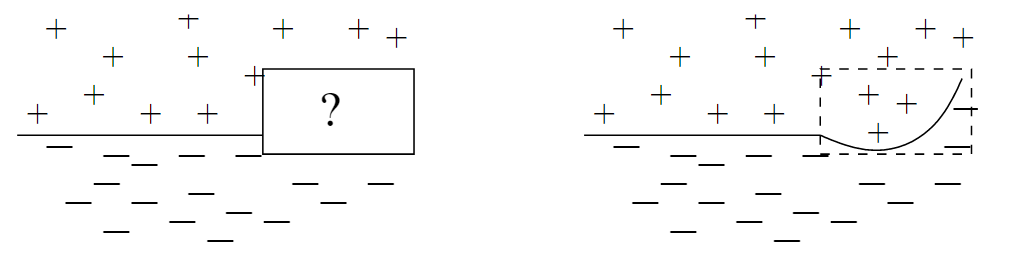
\includegraphics[width=0.8\textwidth]{Figures/ruping_global_local.png}
    \caption{Example of simple global model on the left, and on the right a more simple local model that can be used for interpretability when necessary.}
    \label{fig:ruping}
    \end{figure}

    Later, \citet{Van_Belle2013-ph} address the challenge that some of the highest performing ML models are too complicated to be interpreted. They investigate different `interpretable' and visualization methods in order to understand what opportunities they find. They suggest that there are three methods that help ascertain the level of interpretability and potential utility of models: 1) Map to domain knowledge, 2) Ensure safe operation across the full operational range of model inputs, and 3) Accurately model non-linear effects (compare to categories proposed by \citet{Lipton2016-ug}). They analyze some of the existing methods (nomograms, rule induction, graphical models, data visualization) and point out their weaknesses. They finish by pointing to more recent research in sparse and interpretable models, and suggest that it is a promising line of research. In summary, they discuss that each `interpretable' method has its benefits and weaknesses and there is no method that clearly out-performs any other.

    Similarly, \citet{Caruana2015-za} are interested in predicting the probability that a patient will be re-admitted to the hospital within thirty days. They also mention the trade-off between accuracy and interpretability, and propose a generalized additive model with pairwise interactions ($GA^2M$) model. A generalized additive model (GAM) is generally thought of as interpretable as the effects of individual variables can easily be quantified; however GAMs suffer from low accuracy. In a comparison with other methods, they show that adding pairwise interactions allows the $GA^2M$ model to be as accurate as the current less interpretable methods, while still maintaining reasonable interpretability.

    In a similar vein, \citet{Choi2016-by} modify a recursive attention neural network to remove recurrence on the hidden state vector, and instead add recurrence on the doctor visits and diagnoses. In this way the model is able to predict possible diagnoses in time, and a visualization can be that that indicates the critical visits and diagnoses that lead to that prediction. These methods are promising because it restructures an advanced learning model in a way that useful information can be extracted. This method seems very promising, however, their architecture is dependent on problems with similar properties, meaning that their approach would need to be re-implemented by an expert to be used in another situation.

    \citet{Abdollahi2016-vn} construct a conditional restricted Boltzmann machine (RBM) in order to create a collaborative filtering algorithm, that can suggest `explainable' items, while maintaining accuracy. The challenge is that the RBMs are very accurate collaborative filtering algorithms, but difficult to understand. They make a more explainable version by adding an additional `explainability layer' that encodes which indicates the explainability of an item to a certain user. This method shows how adding an additional element in a model can help add explainability, and this seems to be somewhat of a theme in this section.

    \citet{Ridgeway1998-lv} recognize that boosting methods, or classifiers with voting methods, are very accurate but not interpretable. They propose boosting by `weight of evidence' (WoE), where WoE refers to having a weight that indicates whether the observation is positively or negatively correlated to the class. Each weight can then be used to gain some understanding about how the observation affects the classification. They demonstrate its utility using multiple experiments that it has performance on par with AdaBoost, and with a Naive Bayes classifier.  Again, their approach gets at the ability of adding in interpretability components into a model can yield a more interpretable model, while losing very little accuracy.

    \citet{Huysmans2011-th} investigate decision trees, decision tables, propositional if-then rules, and oblique rule sets in order to understand which is the most interpretable and perform an experiment to identify which method works most effectively. The experiment involved interpreting a model and answering questions about what the correct classification would be. They made several interesting observations. First, they confirmed that a model with larger representation leads to lower answer accuracy responses. They found that overall decision trees and decision tables were the most interpretable, but that different tasks made the tree or table more desirable (the layout of the data in a table can be superior for certain `look-up' tasks). 

    One drawback with decision trees is that the rules can get very complicated in a large tree. \citet{Park2016-ld} investigate how to make rules in decision trees more `intuitive'. They propose a method that learns chains of decisions that together increase the ratio of positive class. They present a method that is called $\alpha$-Carving decision Chain (ACDC), and say that it is a greedy alternative to a general framework known as RuleLists (\citet{Wang2015-ww}). 
    Similarly, \citet{Jovanovic2016-gw} use `Tree-Lasso' logistic regression with domain knowledge. Specifically they use medical diagnostic codes to group similar conditions and then use `Tree-Lasso' regression that uses that information to make a more sparse model. \citet{Zycinski2012-jj} also use domain knowledge to structure the data matrix before feature selection and classification. While the work of \citeauthor{Huysmans2011-th} gives some indication about how to choose classifiers for interpretability, \citeauthor{Park2016-ld} points out that to gain \emph{real} interpretability in complex tasks expert knowledge is still needed to make sense of complicated features.

    \citet{Faghmous2014-og} argue that `theory guided data science' is necessary in science applications; for instance, when studying environmental effects, black-box models are of little use. Instead, in order to gain insight they need a theoretical framework, to help highlight causation. Similarly, \citet{Morrison2016-fz} address the situation where an analytical model is available but imperfect. They use a chemical kinetics application where the theoretical reaction equations are well known, and then add a `stochastic operator' over the top of the known model to account for uncertainties. One drawback for these methods is that they require a lot of domain knowledge. However, in the areas of science and engineering where physical models are well understood this type of approach could be useful to indicate the performance of the system with regards to the theoretical model.


\subsubsection{Visualization and Dimensionality Reduction} \label{sec:viz_dr}
    Intuitively, it might make sense to simply show users the inputs, raw data, and/or intermediate processing steps that led to a particular AIA behavior. In many real applications, however, there are too many individual variables for a human to attend to. In such situations, dimensionality reduction (DR) and visualization are tools that can be used to help make a model or data easier to understand. \citet{Venna2007-yj} discusses dimensionality reduction as a tool for data visualization for ML, and reviews many linear and non-linear projection methods. \citet{Vellido2012-nm} also discusses the importance of DR for making ML models interpretable.

    In an interesting application to time series data, \citet{Kadous1999-rx} asks how comprehensible descriptions of multivariate time series can be learned, with the end goal of interpreting Australian sign language. He focuses on reducing the feature space fed into a learning algorithm (i.e. the data was gathered using an instrumented glove), and does so using `parameterized event primitives' (PEPs), which are commonly occurring events or patterns that are expected to occur. He shows that his method reduced test error while also having more comprehensible features. It seems likely that parameterized primitives might be automatically learned. While an interesting application, this would require expert knowledge to extend to other domains. Although it does seem likely that PEPs could be automatically identified in some way.

\subsubsection{Explanation} \label{sec:explanation}
    In the context of POMDP planning, \citet{Lomas2012-ie} recognize that in order for humans to appropriately trust robots they must be able to predict their behavior, and the robot must be able to communicate in order for that to happen. To this end they present the Explaining Robot Actions (ERA) system that interfaces with a model that represents semantic and physically based information, along with other factors. In essence the ERA is a translator between the planner/model and the human. This approach depends on a layered world model that includes semantic information as well as the physical model, but is promising in the respect that the ERA is a separate system that queries the robot. 

    With regards to expert systems \citet{Swartout1983-ko} examines explanation methods. He noted that ``trust in a system is developed not only by the quality of its results, but also by clear description of how they were derived''. Often the data (or knowledge) used to train an expert system is not kept in the system for later use. He proposed a method called `XPLAIN' that not only describes \emph{what} it did, but \emph{why} it did it. It does this by using description facts of the domain and prescriptive principles simultaneously; in essence it learns how to make decisions and how to explain them at the same time. This approach is meant for a  structured problem defined by a domain model and the domain principles, in situations where problems are based mostly in data, this approach would not be applicable.

    \citet{Rouse1986-dz} asked how computer-based decision support systems should be designed in order to help humans cope with their complexity. He suggests that methods need to be designed so as to provide different kinds of information which include: patterns vs. elements, and current vs. projected outcomes or states. This work is important in pointing out that assurances also depend on what the role of the human is and what information they need. This is a manifestation of the teaching and telling assurances discussed in section \ref{sec:teach_tell}.

    This was also investigated to some extent by \citet{Wallace2001-fm} in their work concerning explaining outcomes of constraint solvers. They discuss how to distinguish between `good' and `bad' explanations. In other words, those explanations that facilitate or detract from the user's ability to understand how the explanation actually applies to the solution being explained. They critically ask the question of how explanations should be presented to users (something that \citet{Kuhn1997-qc} explores more formally with regard to framing of uncertain information in decision making). An important consideration is that constraint solves don't take uncertainty into account, in other words they are deterministic which is not the case in many of the more adaptable and capable AIAs.

    \citet{Lacave2002-cu} revisit some of these ideas from the perspective of explaining Bayesian networks. They are concerned with \emph{how} and \emph{why} a system reaches a conclusion. They present three properties of explanation: 1) content (what to explain), 2) communication (how to explain), and 3) adaptation (how to adapt based on who the user is). It is not possible to cover all of the ideas that they present in their paper, but they are key to the idea of designing assurances. Some key points are that they highlight the differences between explaining evidence, the model, or the reasoning. These are three key considerations in making assurances. They also discuss whether an explanation is mean to be a description or for comprehension, as well as whether explanations need to be on a macro or micro scale (as mentioned by \citeauthor{Ruping2006-xj}). They also consider whether explanations should occur by two-way interaction between system and user, by natural language interaction, or by probabilities. Finally, when considering adaptation, they hit on another key point of assurances, which is that in general application not all users will require (or desire) the same kinds of assurances. This paper points out many challenges and considerations in designing assurances, and illustrates that, as with the `No free lunch' theorem, there is no single `best' assurance that will address every possible situation.


\subsubsection{Model Checking} \label{sec:model_checking}
    While assurances behind reasoning processes can be useful in many situations, they are not trustworthy in and of themselves if the models or assumptions they are based on are flawed to begin with. Thus, there is also great interest in providing assurances that the models and assumptions underlying said AIA reasoning processes are, in fact, sound. \citet{Laskey1991-mf} -- with the intention of helping users of `probability based decision aids' by communicating the validity of the model -- notes that it is infeasible to perform a decision theoretic calculation to decide if revision of the model is necessary. She then presents a class of theoretically justified model revision indicators which are based on the idea of constructing a computationally simple alternate model and then to initiate model revision if the likelihood ratio of alternate model becomes too large. 

    \citet{Zagorecki2015-qy}, discusses the `surprise index' introduced by \citet{Habbema1976-xd}, which is the likelihood of a certain measurement given a specific model, which applies nicely to Bayes-nets that have probabilistic descriptions. The major flaw of the surprise index is that it is computationally infeasible due to the possibility (likelihood) of being a non-analytic distribution. \citeauthor{Zagorecki2015-qy} suggest an approximation by using the log-normal distribution to approximate the distribution of values in the joint probability distribution. Another challenge is knowing what a `good' value for the surprise index is since knowing the maximum likelihood of a non-analytic distribution is not an easy problem.

    \citet{Ghosh2016-dl} present a method, in the framework of a practical self-driving car problem, called Trusted Machine Learning (TML). The main approach of TML is to make ML models fit constraints (be trustable). To do this they utilize tools from formal methods to provide theoretical proof of the functionality of the system. They present `model repair' and `data repair' that they can utilize when the current model doesn't match the data, at which point the model and data can be repaired and control can be replanned in order to conform with the formal method specifications. One challenge that presents itself is how to identify the `trustable' constraints, this returns a lot of responsibility to the designer to foresee all possible failures, which is a strong assumption.

\subsubsection{Human-Involved Learning} \label{sec:human_involved}
    Another possible way to make system assure a human user is to use the human in the learning process. \citet{Freitas2006-qo} addressed this point with regards to discovering `interesting' knowledge from data, by comparing two main approaches. Given such large datasets, human users require assistance from complex systems in order to find patterns and other `interesting' insights. He mentions `user-driven' methods that involve a user pointing out `interesting' templates, or in another method general impressions in the form of IF-THEN rules. He compares these methods to other `data-driven' methods that have been used, and cites other research that suggests that data-driven approaches are not very effective in practice. This is a cautionary tale that many times engineering methods to assist humans are not as effective as we would like to believe. Although, the `user-driven' approach may not fair any better when compared over many users, as each user will likely have different preferences. \citet{Chang2017-kl} also consider a similar, scaled up, `user-driven' approach called `Revolt' that crowd-sources the labeling of images. It is able to attain high accuracy labeling, while also exploring new or ambiguous classes that can be ignored with traditional approaches.

\subsubsection{Summary}
Currently, informally designed assurances fall into several different categories listed above. Many methods focus on informing the user how the model/logic works, there is also some concern about predicting future performance. However, this is a survey of many different kinds of AIAs, and analogs for these methods have not been universally adopted, or even developed for some AIAs. Technical challenges exist that make designing assurances very difficult in some cases. Deterministic and non-deterministic systems must be treated differently by algorithms, but can utilize similar methods of communication.

The idea of more simplistic global models paired with more accurate local models is fairly prominent, this idea is similar to how human experts explain approaches to non-experts; as a non-expert desires to know more about a specific concept of a complex idea, more detailed explanation can be provided.

A sobering reminder is that there is not a single assurance that will perform the best in all situations. Generally, having humans more involved (as in visualization, or human-involved learning) helps make the representations/functionality more human-like and thus more trustworthy. Assurances need, at times, to explain models, data, and reasoning. The methods of explanation can vary and \emph{should} vary based on who requires the explanation.

\subsection{Quadrant IV. (Implicit Assurances, Informal Trust Treatment)}\label{sec:q4}
\subsubsection{Safety and Learning under nonstationarity and risk aversion} \label{sec:safety}
    While a fairly high-level treatment, \citet{Amodei2016-xi} are concerned with `AI safety', which is in essence how to make sure that there is no ``unintended and harmful behavior that [emerges] from machine learning systems''. Given this definition, much of the paper discusses concepts that are critical to AIA assurances. Among the more directly applicable topics in the scope of this paper are: safe exploration (how to learn in a safe manner), and robustness to distributional shift (a difference between training data and test data). They also discuss designing objective functions that are more appropriate. To restate more concretely, there is a need to design objective functions that more accurately reflect the true objective function. A popular example (roughly summarized here) from \citet{Bostrom2014-fz} is a robot that has an objective of making paper clips, it then decides to take over the world in order to maximize its resources and ability to make more paper clips. This highlights the point that sometimes over-simplistic objective functions can result in unintended and unsafe behaviors.

    Generally, stationary data (data whose distribution does not change after training) is assumed in supervised ML. \citet{Sugiyama2013-ci} considers what to do when there is `covariate shift' (or when both training and test data change distribution, but their relation does not change between training and test phases), and `class-balance change' (where the class-prior probabilities are different in training and test phases, but the input distribution of each class does not change). They design and present tools that help diagnose and treat those conditions (this is follow on work for some of what is presented in \citet{Quinonero-Candela2009-fj} where they consider dataset shift). A key approach is to use importance sampling, which involves weighting the training loss by the ratio between the probability of the test data and that of the training data.

    \citet{Hadfield-Menell2016-ws}, in considering an AI safety problem, address the problem of verifying that a robot can be turned off, even when it might have an objective function that indicates that disabling the `off-switch' will reduce the chance of failure. This kind of scenario, or something similar, can easily occur with a sufficiently sophisticated and capable AIA, and a complex enough set of objectives that might result in unintended consequences. They propose that one objective would be for the robot to maximize value for the human, and to not assume that it knows how to perfectly measure that value. 

    \citet{Da_Veiga2012-gh} discuss a form of safety where they are concerned with nonparametric classification and regression with constraints. More specifically, they are concerned about learning Gaussian process (GP) models with inequality constraints, and present a method to do this by using conditional expectations of the truncated multivariate normal distribution (or Tallis formulas). This is not the only work that references learning with constrained GPs. It is also not the only work that considers constrained modeling, but it would take too long to review all of those papers. The main claim here is that constrained models are a way to guarantee the properties of a model within some specifications.

    \citet{Garcia2015-rs} perform a survey about safe reinforcement learning (RL). Safety in RL can be critical based on the application, such as an aerospace vehicle that can cost several thousands of dollars. They state that there are two main methods: 1) modifying the optimality criterion with a safety factor, and 2) modification of the exploration process through the incorporation of external knowledge. They also present a hierarchy of approaches and implementations. Some approaches used when modifying the optimality criterion are worst-case, risk-sensitive, and constrained criterion. Whereas, modifying the exploration process is done through using external knowledge, and as well as using risk-directed exploration. Safe RL is a particularly important area that requires assurances, as the systems are designed specifically to evolve without supervision.

    As one example, \citet{Lipton2016-dq} design a reinforcement learner that uses a deep Q-network (DQN) and a `supervised danger model'. Basically, the danger model stores the likelihood of entering a catastrophe state within a `short number of steps', this model can be learned by detecting catastrophes through experience and can be improved over time.  In this way they show that their method, they call `intrinsic fear', is able to overcome the sensitive nature of DQNs. There is a clear limitation of the danger model, in that it does not contain useful information until a catastrophe is detected. 

    \citet{Curran2016-ij}, in a more specific application, asks how a robot can learn when a task is too risky, and then avoid those situations, or ask for help. To do this, they use a hierarchical POMDP planner that explicitly represents failures as additional state-action pairs. In this way the resulting policy can be averse to risk. They say that this method can be especially useful when optimal actions are not straight-forward, and they state that it can use any reward function. It seems that this method might suffer from some of the typical problems of POMDPs, which are computational complexity in high-dimensional state spaces.

\subsubsection{Active Learning} \label{sec:active_learning}
    \citet{Paul2011-vr} is concerned with whether a robot can improve its own performance over time, with the goal of `life-long learning'. They use `perplexity' which is a method first introduced in language models and adapted to work with images. Perplexity, in their application, is a measure that indicates the uncertainty in predicting a single class. Over time, the most perplexing images are stored and used in expanding the sample set. This work is interesting for application in assurances because the ability to quantify something that is perplexing is a predecessor to being able to communicate that to a human user.

    Recently, there have been several papers that attempt to use Gaussian processes (GPs) as a method to actively learn and assign probabilistic classifications (see \citet{MacKay1992-sp,Triebel2016-kj,Triebel2013-ow,Triebel2013-ku,Grimmett2013-gj,Grimmett2016-yc,Berczi2015-rd,Dequaire2016-kh}). The applications surveyed here are all mainly related to image classification and robotics. As with perplexity-based classifiers, the key insight is that if a classifier possesses a measure of uncertainty, then that uncertainty can be used for efficient instance searching, comparison, and learning, as well as reporting a measure of confidence to users. The key property of GPs that makes them an attractive for this purpose is their ability to produce confidence/uncertainty estimates that grow more uncertain away from the training data. That is, GPs have the inherent ability to `know what they don't know', and this information can be readily assessed and conveyed to users, even in high-dimensional reasoning problems. This property of GPs has also found great use in other active learning applications, such as  Bayesian optimization (see \citet{Williams1998-kr}, \citet{Snoek2012-tt}, \citet{Brochu2010-tj}, and \citet{Israelsen2017-zb}).

\subsubsection{Representation learning and Feature Selection} \label{sec:rep_learning}
    Another promising field of research is related to learning representations of data and selecting data features. These two topics are surveyed by \citet{Bengio2013-uv} and \citet{Guyon2003-fj} respectively. From some of the discussion of interpretable models in section \ref{sec:model_interp} we find that representation is important for making interpretable models. Having appropriate representations (i.e. like the ones humans use and understand) is a large step forward in making assurances for humans.

    For instance, in their work related to interpreting molecular signatures \citet{Haury2011-zi} investigate the influence of different feature selection methods on the accuracy, stability and interpretability of molecular signatures. They compared different feature selection methods such as: filter methods, wrapper methods, and ensemble feature selection. They found that the effects of feature learning greatly influenced the results. 

    As another example, \citet{Mikolov2013-lt} studied how to represent words and phrases in a vector format. Using this representation, they are able to perform simple vector operations to understand similar words, and the relative relationships learned. For example the operation $airlines+German$ yields similar entries that include $Lufthansa$. This type of representation encodes information that can be checked and understood by humans. 
    
    How can human understandable features and representations be discovered? This is still an open question. The main question in the representation learning world is how to find the best representations, not necessarily the representation and features that are most human. This is not surprising because human representations and features are not necessarily optimal, and AIAs are being designed to be optimal using other objective functions (arguably more appropriate functions, if humans don't need to understand what is going on).

\subsubsection{Summary}
    The literature surveyed in this section is \emph{not} exhaustive, nor could it reasonably ever claim to be. One thing that should be clear is that in every field where designers want to ensure reliable and correct application of an AIA, there will be assurances that are created. The disciplines selected in this paper are a subset that are aligned with the author's interests in unmanned vehicles.

    The work in this section is easily distinguished from that in Quadrant I because it does not discuss trust in any way. However, it is only subtly different from that in Quadrant III. The research in Quadrant III is explicitly focused on things like interpretability and explanation by direct statement of the authors. Conversely, the research found in this quadrant is only related to trust by those who are familiar with the underlying concepts in this paper. This research is created with the intent of making the AIAs intrinsically more safe, aware of reasoning processes, having better representations in some way, and others. This group unintentionally, creates foundations for trustworthy AIAs. Here are found the researchers who created AIAs with properties, like reliability, that can then be investigated by those who formally acknowledge human-AIA trust in Quadrant I. These are the methods can be turned into explicit assurances by designers who intentionally do so.

